\documentclass[../main/NEMO_manual]{subfiles}

\begin{document}

\chapter{Miscellaneous Topics}
\label{chap:MISC}

\thispagestyle{plain}

\chaptertoc

\paragraph{Changes record} ~\\

{\footnotesize
  \begin{tabularx}{\textwidth}{l||X|X}
    Release & Author(s) & Modifications \\
    \hline
    {\em   4.0} & {\em ...} & {\em ...} \\
    {\em   3.6} & {\em ...} & {\em ...} \\
    {\em   3.4} & {\em ...} & {\em ...} \\
    {\em <=3.4} & {\em ...} & {\em ...}
  \end{tabularx}
}

\clearpage

%% =================================================================================================
\section{Representation of unresolved straits}
\label{sec:MISC_strait}

In climate modeling, it often occurs that a crucial connections between water masses is broken as
the grid mesh is too coarse to resolve narrow straits.
For example, coarse grid spacing typically closes off the Mediterranean from the Atlantic at
the Strait of Gibraltar.
In this case, it is important for climate models to include the effects of salty water entering the Atlantic from
the Mediterranean.
Likewise, it is important for the Mediterranean to replenish its supply of water from the Atlantic to
balance the net evaporation occurring over the Mediterranean region.
This problem occurs even in eddy permitting simulations.
For example, in ORCA 1/4\deg\ several straits of the Indonesian archipelago (Ombai, Lombok...)
are much narrow than even a single ocean grid-point.

We describe briefly here the two methods that can be used in \NEMO\ to handle such
improperly resolved straits. The methods consist of opening the strait while ensuring
that the mass exchanges through the strait are not too large by either artificially
reducing the cross-sectional area of the strait grid-cells or, locally increasing the
lateral friction.

%% =================================================================================================
\subsection{Hand made geometry changes}
\label{subsec:MISC_strait_hand}

The first method involves reducing the scale factor in the cross-strait direction to a
value in better agreement with the true mean width of the strait
(\autoref{fig:MISC_strait_hand}).  This technique is sometime called "partially open face"
or "partially closed cells".  The key issue here is only to reduce the faces of $T$-cell
(\ie\ change the value of the horizontal scale factors at $u$- or $v$-point) but not the
volume of the $T$-cell.  Indeed, reducing the volume of strait $T$-cell can easily produce
a numerical instability at that grid point which would require a reduction of the model
time step.  Thus to instigate a local change in the width of a Strait requires two steps:

\begin{itemize}

\item Add \texttt{e1e2u} and \texttt{e1e2v} arrays to the \np{cn_domcfg}{cn\_domcfg} file. These 2D
arrays should contain the products of the unaltered values of: $\texttt{e1u}*\texttt{e2u}$
and $\texttt{e1u}*\texttt{e2v}$ respectively. That is the original surface areas of $u$-
and $v$- cells respectively.  These areas are usually defined by the corresponding product
within the \NEMO\ code but the presence of \texttt{e1e2u} and \texttt{e1e2v} in the
\np{cn_domcfg}{cn\_domcfg} file will suppress this calculation and use the supplied fields instead.
If the model domain is provided by user-supplied code in \mdl{usrdef\_hgr}, then this
routine should also return \texttt{e1e2u} and \texttt{e1e2v} and set the integer return
argument \texttt{ie1e2u\_v} to a non-zero value. Values other than 0 for this argument
will suppress the calculation of the areas.

\item Change values of \texttt{e2u} or \texttt{e1v} (either in the \np{cn_domcfg}{cn\_domcfg} file or
via code in  \mdl{usrdef\_hgr}), whereever a Strait reduction is required. The choice of
whether to alter \texttt{e2u} or \texttt{e1v} depends. respectively,  on whether the
Strait in question is North-South orientated (\eg\ Gibraltar) or East-West orientated (\eg
Lombok).

\end{itemize}

The second method is to increase the viscous boundary layer thickness by a local increase
of the fmask value at the coast. This method can also be effective in wider passages.  The
concept is illustarted in the second part of  \autoref{fig:MISC_strait_hand} and changes
to specific locations can be coded in \mdl{usrdef\_fmask}. The \forcode{usr_def_fmask}
routine is always called after \texttt{fmask} has been defined according to the choice of
lateral boundary condition as discussed in \autoref{sec:LBC_coast}. The default version of
\mdl{usrdef\_fmask} contains settings specific to ORCA2 and ORCA1 configurations. These are
meant as examples only; it is up to the user to verify settings and provide alternatives
for their own configurations. The default \forcode{usr_def_fmask} makes no changes to
\texttt{fmask} for any other configuration.

\begin{figure}[!tbp]
  \centering
  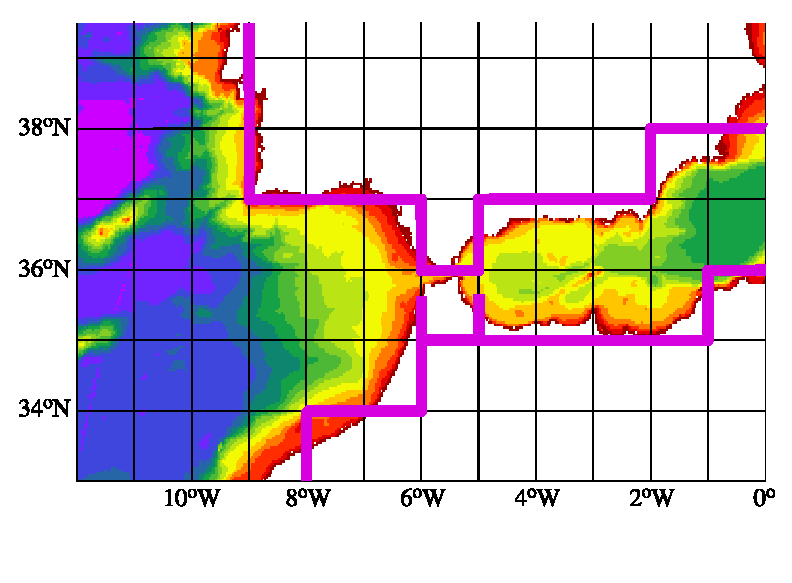
\includegraphics[width=0.66\textwidth]{MISC_Gibraltar}
  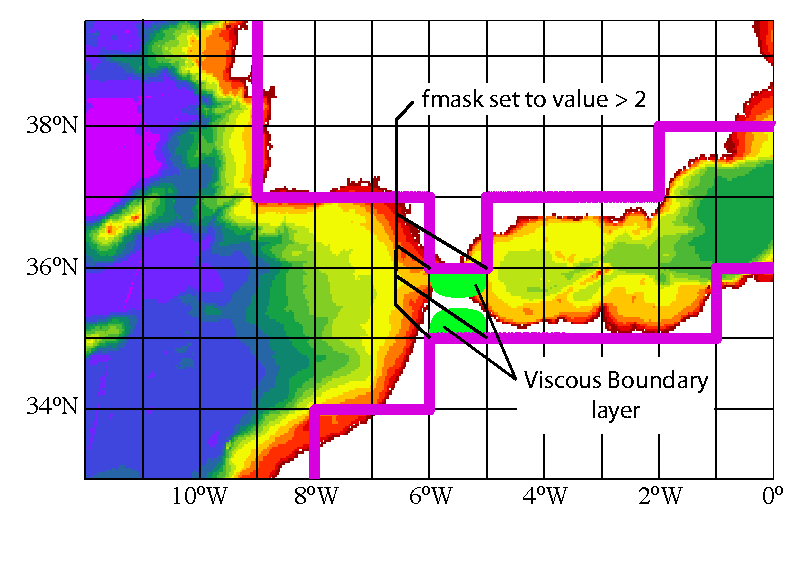
\includegraphics[width=0.66\textwidth]{MISC_Gibraltar2}
  \caption[Two methods to defined the Gibraltar strait]{
    Example of the Gibraltar strait defined in a 1\deg\ $\times$ 1\deg\ mesh.
    \textit{Top}: using partially open cells.
    The meridional scale factor at $v$-point is reduced on both sides of the strait to
    account for the real width of the strait (about 20 km).
    Note that the scale factors of the strait $T$-point remains unchanged.
    \textit{Bottom}: using viscous boundary layers.
    The four fmask parameters along the strait coastlines are set to a value larger than 4,
    \ie\ "strong" no-slip case (see \autoref{fig:LBC_shlat}) creating a large viscous boundary layer
    that allows a reduced transport through the strait.}
  \label{fig:MISC_strait_hand}
\end{figure}

\begin{figure}[!tbp]
  \centering
  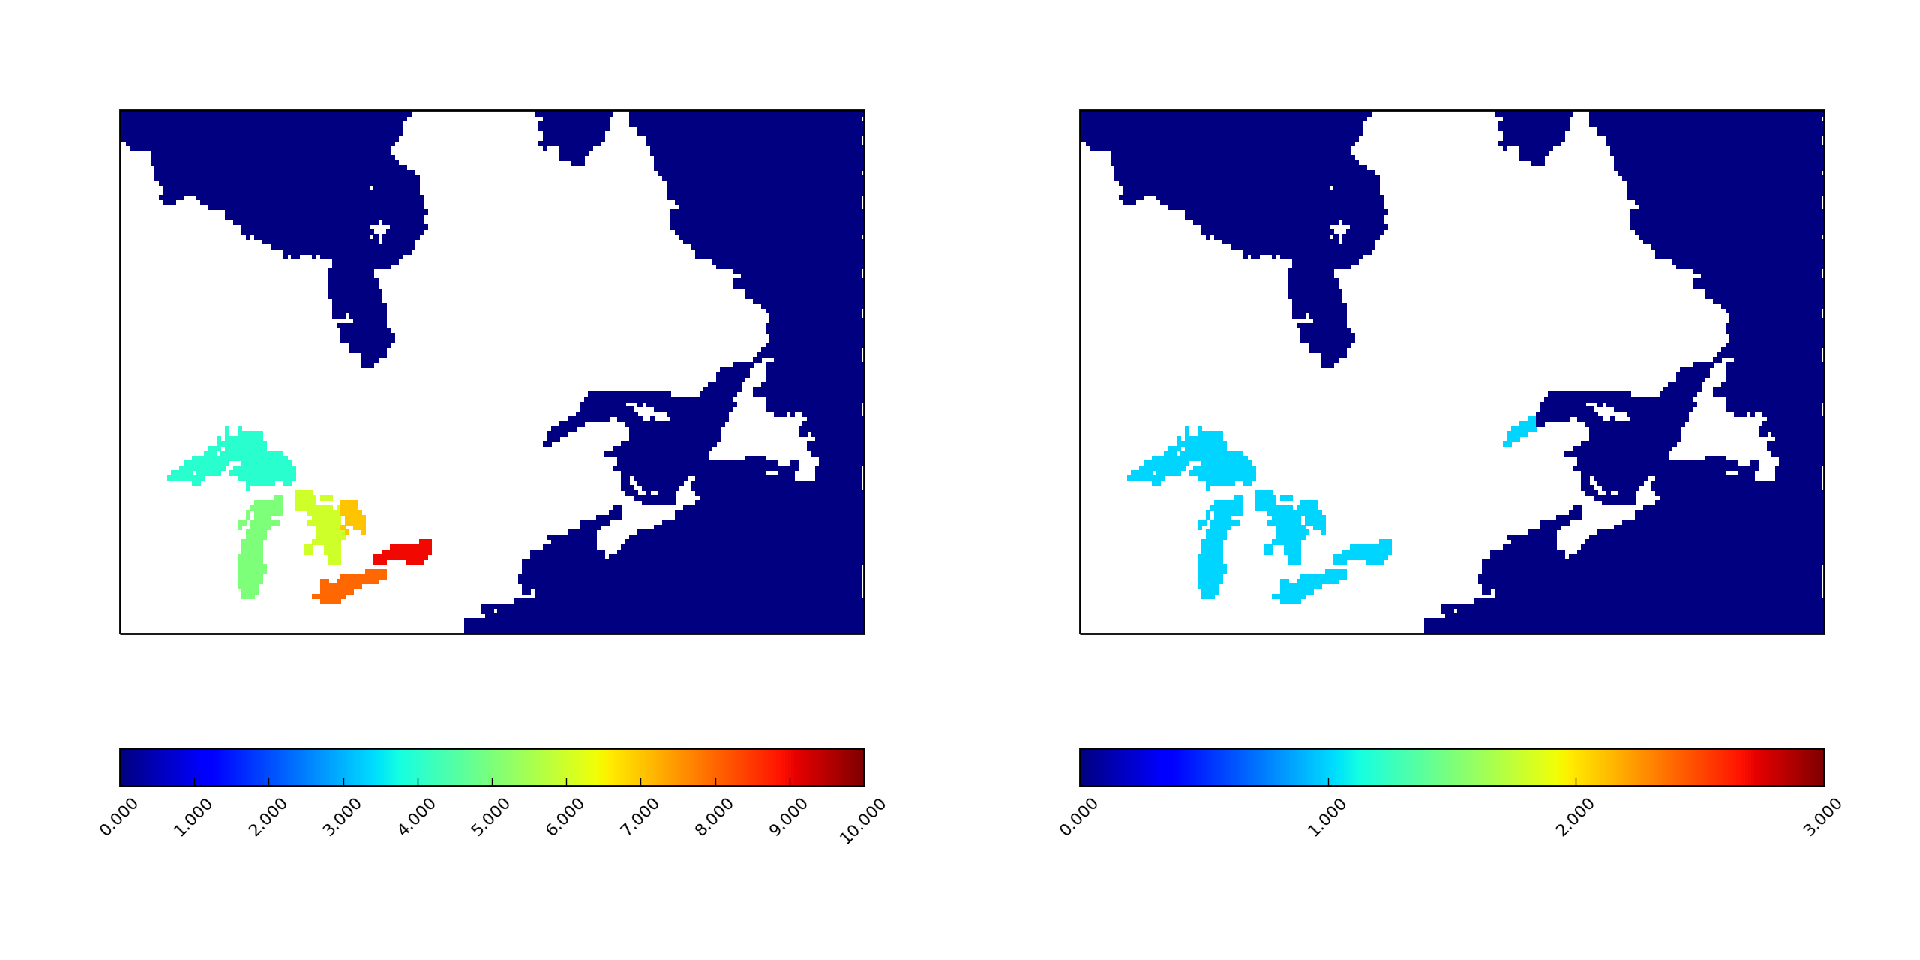
\includegraphics[width=0.66\textwidth]{MISC_closea_mask_example}
  \caption[Mask fields for the \protect\mdl{closea} module]{
    Example of mask fields for the \protect\mdl{closea} module.
    \textit{Left}: a closea\_mask field;
    \textit{Right}: a closea\_mask\_rnf field.
    In this example, if \protect\np{ln_closea}{ln\_closea} is set to \forcode{.true.},
    the mean freshwater flux over each of the American Great Lakes will be set to zero,
    and the total residual for all the lakes, if negative, will be put into
    the St Laurence Seaway in the area shown.}
  \label{fig:MISC_closea_mask_example}
\end{figure}

%% =================================================================================================
\section[Closed seas (\textit{closea.F90})]{Closed seas (\protect\mdl{closea})}
\label{sec:MISC_closea}

Some configurations include inland seas and lakes as ocean
points. This is particularly the case for configurations that are
coupled to an atmosphere model where one might want to include inland
seas and lakes as ocean model points in order to provide a better
bottom boundary condition for the atmosphere. However there is no
route for freshwater to run off from the lakes to the ocean and this
can lead to large drifts in the sea surface height over the lakes. The
closea module provides options to either fill in closed seas and lakes
at run time, or to set the net surface freshwater flux for each lake
to zero and put the residual flux into the ocean.

Prior to \NEMO\ 4 the locations of inland seas and lakes was set via
hardcoded indices for various ORCA configurations. From \NEMO\ 4 onwards
the inland seas and lakes are defined using mask fields in the
domain configuration file. The options are as follows.

\begin{enumerate}
\item {{\bfseries No ``closea\_mask'' field is included in domain configuration
  file.} In this case the closea module does nothing.}

\item {{\bfseries A field called closea\_mask is included in the domain
configuration file and ln\_closea=.false. in namelist namcfg.} In this
case the inland seas defined by the closea\_mask field are filled in
(turned to land points) at run time. That is every point in
closea\_mask that is nonzero is set to be a land point.}

\item {{\bfseries A field called closea\_mask is included in the domain
configuration file and ln\_closea=.true. in namelist namcfg.} Each
inland sea or group of inland seas is set to a positive integer value
in the closea\_mask field (see \autoref{fig:MISC_closea_mask_example}
for an example). The net surface flux over each inland sea or group of
inland seas is set to zero each timestep and the residual flux is
distributed over the global ocean (ie. all ocean points where
closea\_mask is zero).}

\item {{\bfseries Fields called closea\_mask and closea\_mask\_rnf are
included in the domain configuration file and ln\_closea=.true. in
namelist namcfg.} This option works as for option 3, except that if
the net surface flux over an inland sea is negative (net
precipitation) it is put into the ocean at specified runoff points. A
net positive surface flux (net evaporation) is still spread over the
global ocean. The mapping from inland seas to runoff points is defined
by the closea\_mask\_rnf field. Each mapping is defined by a positive
integer value for the inland sea(s) and the corresponding runoff
points. An example is given in
\autoref{fig:MISC_closea_mask_example}. If no mapping is provided for a
particular inland sea then the residual is spread over the global
ocean.}

\item {{\bfseries Fields called closea\_mask and closea\_mask\_emp are
included in the domain configuration file and ln\_closea=.true. in
namelist namcfg.} This option works the same as option 4 except that
the nonzero net surface flux is sent to the ocean at the specified
runoff points regardless of whether it is positive or negative. The
mapping from inland seas to runoff points in this case is defined by
the closea\_mask\_emp field.}
\end{enumerate}

There is a python routine to create the closea\_mask fields and append
them to the domain configuration file in the utils/tools/DOMAINcfg directory.

%% =================================================================================================
\section{Sub-domain functionality}
\label{sec:MISC_zoom}

%% =================================================================================================
\subsection{Simple subsetting of input files via NetCDF attributes}

The extended grids for use with the under-shelf ice cavities will result in redundant rows
around Antarctica if the ice cavities are not active.  A simple mechanism for subsetting
input files associated with the extended domains has been implemented to avoid the need to
maintain different sets of input fields for use with or without active ice cavities.  This
subsetting operates for the j-direction only and works by optionally looking for and using
a global file attribute (named: \np{open_ocean_jstart}{open\_ocean\_jstart}) to determine the starting j-row
for input.  The use of this option is best explained with an example:
\medskip

\noindent Consider an ORCA1
configuration using the extended grid domain configuration file: \ifile{eORCA1\_domcfg.nc}
This file define a horizontal domain of 362x332.  The first row with
open ocean wet points in the non-isf bathymetry for this set is row 42 (\fortran\ indexing)
then the formally correct setting for \np{open_ocean_jstart}{open\_ocean\_jstart} is 41.  Using this value as
the first row to be read will result in a 362x292 domain which is the same size as the
original ORCA1 domain.  Thus the extended domain configuration file can be used with all
the original input files for ORCA1 if the ice cavities are not active (\np{ln\_isfcav =
.false.}).  Full instructions for achieving this are:

\begin{itemize}
\item Add the new attribute to any input files requiring a j-row offset, i.e:
\begin{cmds}
ncatted  -a open_ocean_jstart,global,a,d,41 eORCA1_domcfg.nc
\end{cmds}

\item Add the logical switch \np{ln_use_jattr}{ln\_use\_jattr} to \nam{cfg}{cfg} in the configuration
namelist (if it is not already there) and set \forcode{.true.}
\end{itemize}

\noindent Note that with this option, the j-size of the global domain is (extended
j-size minus \np{open_ocean_jstart}{open\_ocean\_jstart} + 1 ) and this must match the \texttt{jpjglo} value
for the configuration. This means an alternative version of \ifile{eORCA1\_domcfg.nc} must
be created for when \np{ln_use_jattr}{ln\_use\_jattr} is active. The \texttt{ncap2} tool provides a
convenient way of achieving this:

\begin{cmds}
ncap2 -s 'jpjglo=292' eORCA1_domcfg.nc nORCA1_domcfg.nc
\end{cmds}

The domain configuration file is unique in this respect since it also contains the value of \jp{jpjglo}
that is read and used by the model.
Any other global, 2D and 3D, netcdf, input field can be prepared for use in a reduced domain by adding the
\texttt{open\_ocean\_jstart} attribute to the file's global attributes.
In particular this is true for any field that is read by \NEMO\ using the following optional argument to
the appropriate call to \np{iom_get}{iom\_get}.

\begin{forlines}
lrowattr=ln_use_jattr
\end{forlines}

Currently, only the domain configuration variables make use of this optional argument so
this facility is of little practical use except for tests where no other external input
files are needed or you wish to use an extended domain configuration with inputs from
earlier, non-extended configurations. Alternatively, it should be possible to exclude
empty rows for extended domain, forced ocean runs using interpolation on the fly, by
adding the optional argument to \texttt{iom\_get} calls for the weights and initial
conditions. Experimenting with this remains an exercise for the user.

%% =================================================================================================
\section[Accuracy and reproducibility (\textit{lib\_fortran.F90})]{Accuracy and reproducibility (\protect\mdl{lib\_fortran})}
\label{sec:MISC_fortran}

%% =================================================================================================
\subsection[Issues with intrinsinc SIGN function (\texttt{\textbf{key\_nosignedzero}})]{Issues with intrinsinc SIGN function (\protect\key{nosignedzero})}
\label{subsec:MISC_sign}

The SIGN(A, B) is the \fortran\ intrinsic function delivers the magnitude of A with the sign of B.
For example, SIGN(-3.0,2.0) has the value 3.0.
The problematic case is when the second argument is zero, because, on platforms that support IEEE arithmetic,
zero is actually a signed number.
There is a positive zero and a negative zero.

In \fninety, the processor was required always to deliver a positive result for SIGN(A, B) if B was zero.
Nevertheless, in \fninety, the processor is allowed to do the correct thing and deliver ABS(A) when
B is a positive zero and -ABS(A) when B is a negative zero.
This change in the specification becomes apparent only when B is of type real, and is zero,
and the processor is capable of distinguishing between positive and negative zero,
and B is negative real zero.
Then SIGN delivers a negative result where, under \fninety\ rules, it used to return a positive result.
This change may be especially sensitive for the ice model,
so we overwrite the intrinsinc function with our own function simply performing :   \\
\verb?   IF( B >= 0.e0 ) THEN   ;   SIGN(A,B) = ABS(A)  ?    \\
\verb?   ELSE                   ;   SIGN(A,B) =-ABS(A)     ?  \\
\verb?   ENDIF    ? \\
This feature can be found in \mdl{lib\_fortran} module and is effective when \key{nosignedzero} is defined.
We use a CPP key as the overwritting of a intrinsic function can present performance issues with
some computers/compilers.

%% =================================================================================================
\subsection{MPP reproducibility}
\label{subsec:MISC_glosum}

The numerical reproducibility of simulations on distributed memory parallel computers is a critical issue.
In particular, within \NEMO\ global summation of distributed arrays is most susceptible to rounding errors,
and their propagation and accumulation cause uncertainty in final simulation reproducibility on
different numbers of processors.
To avoid so, based on \citet{he.ding_JS01} review of different technics,
we use a so called self-compensated summation method.
The idea is to estimate the roundoff error, store it in a buffer, and then add it back in the next addition.

Suppose we need to calculate $b = a_1 + a_2 + a_3$.
The following algorithm will allow to split the sum in two
($sum_1 = a_{1} + a_{2}$ and $b = sum_2 = sum_1 + a_3$) with exactly the same rounding errors as
the sum performed all at once.
\begin{align*}
	sum_1 \ \  &= a_1 + a_2 \\
	error_1     &= a_2 + ( a_1 - sum_1 ) \\
	sum_2 \ \  &= sum_1 + a_3 + error_1 \\
	error_2     &= a_3 + error_1 + ( sum_1 - sum_2 ) \\
	b \qquad \ &= sum_2 \\
\end{align*}
An example of this feature can be found in \mdl{lib\_fortran} module.
It is systematicallt used in glob\_sum function (summation over the entire basin excluding duplicated rows and
columns due to cyclic or north fold boundary condition as well as overlap MPP areas).
The self-compensated summation method should be used in all summation in i- and/or j-direction.
See \mdl{closea} module for an example.
Note also that this implementation may be sensitive to the optimization level.

%% =================================================================================================
\subsection{MPP scalability}
\label{subsec:MISC_mppsca}

The default method of communicating values across the north-fold in distributed memory applications (\key{mpp\_mpi})
uses a \textsc{MPI\_ALLGATHER} function to exchange values from each processing region in
the northern row with every other processing region in the northern row.
This enables a global width array containing the top 4 rows to be collated on every northern row processor and then
folded with a simple algorithm.
Although conceptually simple, this "All to All" communication will hamper performance scalability for
large numbers of northern row processors.
From version 3.4 onwards an alternative method is available which only performs direct "Peer to Peer" communications
between each processor and its immediate "neighbours" across the fold line.
This is achieved by using the default \textsc{MPI\_ALLGATHER} method during initialisation to
help identify the "active" neighbours.
Stored lists of these neighbours are then used in all subsequent north-fold exchanges to
restrict exchanges to those between associated regions.
The collated global width array for each region is thus only partially filled but is guaranteed to
be set at all the locations actually required by each individual for the fold operation.
This alternative method should give identical results to the default \textsc{ALLGATHER} method and
is recommended for large values of \np{jpni}{jpni}.
The new method is activated by setting \np{ln_nnogather}{ln\_nnogather} to be true (\nam{mpp}{mpp}).
The reproducibility of results using the two methods should be confirmed for each new,
non-reference configuration.

%% =================================================================================================
\section{Model optimisation, control print and benchmark}
\label{sec:MISC_opt}

\begin{listing}
  \nlst{namctl}
  \caption{\forcode{&namctl}}
  \label{lst:namctl}
\end{listing}

Options are defined through the  \nam{ctl}{ctl} namelist variables.

%% =================================================================================================
\subsection{Vector optimisation}

\key{vectopt\_loop} enables the internal loops to collapse.
This is very a very efficient way to increase the length of vector calculations and thus
to speed up the model on vector computers.

% Add here also one word on NPROMA technique that has been found useless, since compiler have made significant progress during the last decade.

% Add also one word on NEC specific optimisation (Novercheck option for example)

%% =================================================================================================
\subsection{Control print}

The \np{ln_ctl}{ln\_ctl} switch was originally used as a debugging option in two modes:

\begin{enumerate}
\item {\np{ln_ctl}{ln\_ctl}: compute and print the trends averaged over the interior domain in all TRA, DYN, LDF and
ZDF modules.
This option is very helpful when diagnosing the origin of an undesired change in model results. }

\item {also \np{ln_ctl}{ln\_ctl} but using the nictl and njctl namelist parameters to check the source of differences between
mono and multi processor runs.}
\end{enumerate}

However, in recent versions it has also been used to force all processors to assume the
reporting role. Thus when \np{ln_ctl}{ln\_ctl} is true all processors produce their own versions
of files such as: ocean.output, layout.dat, etc.  All such files, beyond the the normal
reporting processor (narea == 1), are named with a \_XXXX extension to their name, where
XXXX is a 4-digit area number (with leading zeros, if required). Other reporting files
such as run.stat (and its netCDF counterpart: run.stat.nc) and tracer.stat contain global
information and are only ever produced by the reporting master (narea == 1). For version
4.0 a start has been made to return \np{ln_ctl}{ln\_ctl} to its original function by introducing
a new control structure which allows finer control over which files are produced. This
feature is still evolving but it does already allow the user to: select individually the
production of run.stat and tracer.stat files and to toggle the production of other files
on processors other than the reporting master. These other reporters can be a simple
subset of processors as defined by a minimum, maximum and incremental processor number.

Note, that production of the run.stat and tracer.stat files require global communications.
For run.stat, these are global min and max operations to find metrics such as the gloabl
maximum velocity. For tracer.stat these are global sums of tracer fields. To improve model
performance these operations are disabled by default and, where necessary, any use of the
global values have been replaced with local calculations. For example, checks on the CFL
criterion are now done on the local domain and only reported if a breach is detected.

Experienced users may wish to still monitor this information as a check on model progress.
If so, the best compromise will be to activate the files with:

\begin{verbatim}
     sn_cfctl%l_config = .TRUE.
       sn_cfctl%l_runstat = .TRUE.
       sn_cfctl%l_trcstat = .TRUE.
\end{verbatim}

and to use the new time increment setting to ensure the values are collected and reported
at a suitably long interval. For example:

\begin{verbatim}
       sn_cfctl%ptimincr  = 25
\end{verbatim}

will carry out the global communications and write the information every 25 timesteps. This
increment also applies to the time.step file which is otherwise updated every timestep.

\subinc{
\clearpage

%% Bibliography
\phantomsection
\addcontentsline{toc}{chapter}{Bibliography}
\lohead{Bibliography} \rehead{Bibliography}
\bibliography{../main/bibliography}

\clearpage

%% Indexes
\phantomsection
\addcontentsline{toc}{chapter}{Indexes}
\lohead{Indexes} \rehead{Indexes}
\printindex[blocks]
\printindex[keys]
\printindex[modules]
\printindex[parameters]
\printindex[subroutines]
}

\end{document}
